\documentclass[conference]{IEEEtran}
\IEEEoverridecommandlockouts

\usepackage{cite}
\usepackage{amsmath,amssymb,amsfonts}
\usepackage{algorithmic}
\usepackage{graphicx}
\usepackage{textcomp}
\usepackage{xcolor}
\usepackage{url}
\usepackage{array}
\usepackage{booktabs}
\usepackage{tabularx} % Added for automatic column width calculation
\usepackage{tikz}
\usetikzlibrary{arrows.meta,positioning,shapes.geometric}
\newcolumntype{Y}{>{\centering\arraybackslash}X}
\newcolumntype{P}[1]{>{\centering\arraybackslash}p{#1}}
\setlength{\tabcolsep}{4pt}
\renewcommand{\arraystretch}{1.2}

\def\BibTeX{{\rm B\kern-.05em{\sc i\kern-.025em b}\kern-.08em
    T\kern-.1667em\lower.7ex\hbox{E}\kern-.125emX}}

\begin{document}

\title{Resource-Aware Adaptive Scheduling for Online Code Judge Systems: From Bare-Metal Calibration to Hyperscale Cloud Provisioning}

\author{
\begin{tabular*}{\textwidth}{@{\extracolsep{\fill}}ccc@{}}
\begin{tabular}{c}
{\normalfont Bharath Aashish R}\\
{\itshape\small Dept. of Computer Science \& Engineering}\\
{\itshape\small Easwari Engineering College}\\
{\small Chennai, India}\\
{\small bharathaashish@gmail.com}
\end{tabular} & & \begin{tabular}{c}
{\normalfont Dhanush M}\\
{\itshape\small Dept. of Computer Science \& Engineering}\\
{\itshape\small Easwari Engineering College}\\
{\small Chennai, India}\\
{\small dhanush.m.0808@gmail.com}
\end{tabular}\\[1.4ex]
\begin{tabular}{c}
{\normalfont Hemanthkumar K}\\
{\itshape\small Dept. of Computer Science \& Engineering}\\
{\itshape\small Easwari Engineering College}\\
{\small Chennai, India}\\
{\small hemanthkumar2k04@gmail.com}
\end{tabular} & \begin{tabular}{c}
{\normalfont Iniyaa P}\\
{\itshape\small Dept. of Computer Science \& Engineering}\\
{\itshape\small Easwari Engineering College}\\
{\small Chennai, India}\\
{\small iniyaapaari@gmail.com}
\end{tabular} & \begin{tabular}{c}
{\normalfont Indumathy P}\\
{\itshape\small Assistant Professor, Dept. of CSE}\\
{\itshape\small Easwari Engineering College}\\
{\small Chennai, India}\\
{\small indumathy.p@eec.srmrmp.edu.in}
\end{tabular}\\
\end{tabular*}
}

\maketitle

\begin{abstract}
Online Code Judge (OJ) platforms commonly isolate submissions by assigning every one of them the same worst-case resource ceiling, typically 2048~MiB of RAM and 2.0 CPU cores. This keeps memory-intensive dynamic programming tasks from triggering an Out-Of-Memory (OOM) kill, but it does so at a real cost: in our 72-run CodeNet benchmark, 78.7\% of correctly-executing submissions used less than 25~MiB of resident set size (RSS), well below what each one was allocated, and the mean was 43.1~MiB against a 2048~MiB ceiling. On fixed, non-elastic on-premises hardware, such as ICPC contest workstations or university exam servers, this static ceiling bounds concurrency to $K = \lfloor (M_{\mathrm{host}} - M_{\mathrm{os}}) / R_{\mathrm{static}} \rfloor$, and during a submission rush that limit produces queue backlogs of several seconds. Applying the same fixed ceiling in a cloud deployment increases reserved infrastructure cost by roughly 16$\times$ in our projection.

This paper evaluates RAAS-OCJS (Resource-Aware Adaptive Scheduling for Online Contest Judge Systems), which replaces the fixed ceiling with dynamic, tiered scheduling governed by a Linux cgroups~v2 soft watermark ($\theta = 70\%$, corresponding to 179.2~MiB of a 256~MiB baseline tier). Our evaluation has two stages. First, we captured real kernel-level memory and CPU profiles on a dedicated bare-metal testbed (13th Gen Intel Core i5-13420H, 12 threads, 15~GiB usable RAM, Fedora Linux), in a 72-run live benchmark over problems drawn from IBM Project CodeNet \cite{puri2021codenet} and Hugging Face \texttt{deepmind/code\_contests} \cite{li2022alphacode}, across C++, Python, Java, and C. Second, we used those measured profiles to drive a 10,000-submission contest simulation and a further theoretical projection onto AWS EC2 cloud provisioning costs; neither the 10,000-submission run nor the cloud figures were executed on live infrastructure, and we report them as simulation and projection results rather than deployment measurements. Third, we executed a complete 80-run live matrix (5 problems $\times$ 4 languages $\times$ 4 strategies) on the deployed 256~MiB tier, all 80 of which returned correct verdicts. Alongside the simulation we executed a complete 80-run live matrix (5 problems $\times$ 4 languages $\times$ 4 strategies) on the same testbed, of which all 80 returned correct verdicts.

The live 80-run matrix shows that tier selection carries no measurable CPU cost (4.2\% spread across strategies) and that live promotion fired in 8 of 8 eligible cases, in 259--817~ms depending on the language runtime, with every promoted submission still correct. It also exposes a limitation we report rather than conceal: the predictive classifier alone routed all four heavy-workload languages to the light tier and never promoted, with the JVM clearing the hard limit by only 24.3~MB. Prediction reduces how often a submission is constrained; the kernel watermark is what keeps the constrained ones correct.

Seeded with our measured profiles, the 10,000-submission simulation shows RAAS-OCJS reclaiming 10,316.25~GB of RAM (a 51.58\% reduction) and cutting CPU core-hours by 20.26\% relative to the static baseline. In the simulated 500-submission freeze rush, adaptive tiering eliminates queue wait time (14,590.1~ms down to 0.0~ms) and cuts P95 turnaround latency by 21.4$\times$ (1,320.2~ms vs. 28,238.5~ms). The cloud cost projection, built on these same profiles, works out to a 16.0$\times$ reduction in base pod memory and an 88.9\% reduction in required VM instances, worth USD~21.76 per hour at \texttt{c6i.4xlarge} pricing, under the assumptions stated in Section~V. We also report a measured boundary test at a 128~MiB tier limit that isolates the JVM's tier-sizing requirement, and outline directions for future, language-aware tier sizing.
\end{abstract}

\begin{IEEEkeywords}
Online judge systems, resource-aware scheduling, adaptive cgroups, soft watermark, AST analysis, XGBoost, cloud provisioning, queue latency.
\end{IEEEkeywords}

\section{Introduction}
Online code judge (OJ) platforms underpin computer science education, competitive programming contests (such as the International Collegiate Programming Contest, ICPC), and automated technical interviews \cite{wasik2018survey}. As programming education expands, judges must evaluate thousands of code submissions concurrently while guaranteeing deterministic isolation and strict sandboxing. Existing research has addressed this computational demand primarily through infrastructure-level expansion: deploying elastic cloud clusters \cite{pan2022cloud}, distributing jobs over message queues \cite{song2025idl}, or deploying geographically replicated edge judges \cite{wang2021metaoj}.

These approaches share a fundamental, costly assumption: \textit{every submission, regardless of its computational structure, receives identical, worst-case sandbox resource ceilings} (typically 2048~MiB of RAM and 2.0 CPU cores).

This convention creates three practical problems:
\begin{itemize}
    \item \textbf{Resource Underutilization}: Most contest submissions implement standard algorithmic logic (e.g., prefix sums, two pointers, greedy string scans), and in our measurements these typically required 5~MiB to 25~MiB of resident set size (RSS). Reserving 2048~MiB for each of them leaves most of that allocation idle.
    \item \textbf{Concurrency Starvation on Fixed Hardware}: In air-gapped regional contests or campus lab servers, where external cloud bursting is not an option, the judge runs on a fixed physical machine (e.g., 15~GiB usable RAM). A static 2048~MiB quota limits concurrency to 7 execution slots on that host, which produces queue backlogs and submission timeouts during a scoreboard freeze rush.
    \item \textbf{Cloud Billing Inflation}: Public cloud providers (AWS, GCP, Azure) bill by reserved node capacity, not actual usage. Provisioning for the worst case means contest organizers end up renting far more virtual machines than the workload actually needs; our projection in Section~VI estimates an 88.9\% reduction in required instances.
\end{itemize}

To address this, this paper presents \textbf{RAAS-OCJS} (Resource-Aware Adaptive Scheduling for Online Contest Judge Systems), which introduces a two-tier execution framework:
\begin{enumerate}
    \item A lightweight default sandbox (\textbf{Tier 1: 256~MiB RAM, 1.0 CPU core}) that safely hosts the large majority of incoming submissions;
    \item An active Linux cgroup~v2 soft watermark ($\theta = 70\%$, corresponding to 179.2~MiB of a 256~MiB baseline tier) that detects high memory utilization in-flight and executes live, mid-execution container limit expansion, lifting the container to uncapped memory and CPU without restarting the container or losing process state. Measured end-to-end from submission acceptance to completed promotion, this takes 259~ms to 817~ms depending on the language runtime, and 100\% of promoted submissions in our evaluation still returned a correct verdict;
    \item An offline Machine Learning (XGBoost) classifier driven by Tree-sitter Abstract Syntax Tree (AST) static structural metrics that predicts memory-intensive jobs upon ingress.
\end{enumerate}



\section{Theoretical Model and Queueing Architecture}

\subsection{Mathematical Formulation of Memory Waste}
Let $S = \{s_1, s_2, \dots, s_N\}$ denote a sequence of $N$ submissions entering an online judge. Under static overprovisioning, the system assigns a fixed resource allocation:
\begin{equation}
R_{\mathrm{alloc}}(s_i) = R_{\mathrm{max}}, \quad \forall s_i \in S
\end{equation}
where $R_{\mathrm{max}}$ is typically 2048~MiB. Let $R_{\mathrm{peak}}(s_i)$ denote the actual peak resident set size (RSS) consumed by $s_i$. The unallocated, wasted memory for submission $s_i$ is:
\begin{equation}
\mathrm{Waste}(s_i) = R_{\mathrm{alloc}}(s_i) - R_{\mathrm{peak}}(s_i)
\end{equation}
The system-wide memory waste percentage $W$ across a contest of $N$ submissions is:
\begin{equation}
W = \left[ \frac{\sum_{i=1}^N \left( R_{\mathrm{alloc}}(s_i) - R_{\mathrm{peak}}(s_i) \right)}{\sum_{i=1}^N R_{\mathrm{alloc}}(s_i)} \right] \times 100\%
\end{equation}
Because introductory and greedy problems require merely 6~MiB to 25~MiB, $R_{\mathrm{peak}}(s_i) \ll R_{\mathrm{max}}$. Our simulation of this waste model reports 97.51\% allocated memory wasted under the static baseline.

\subsection{Concurrency Capacity and Queueing Collapse}
On a host with usable physical RAM $M_{\mathrm{host}}$ and operating system reserve $M_{\mathrm{os}}$, the safe concurrency capacity $K$ under non-overcommitted execution is:
\begin{equation}
K_{\mathrm{safe}} = \left\lfloor \frac{M_{\mathrm{host}} - M_{\mathrm{os}}}{R_{\mathrm{alloc}}} \right\rfloor
\end{equation}
On our 15~GiB physical calibration host ($M_{\mathrm{host}} = 15,360$~MiB, $M_{\mathrm{os}} = 1,024$~MiB), baseline static allocation ($R_{\mathrm{max}} = 2048$~MiB) limits concurrency strictly to:
\begin{equation}
K_{\mathrm{safe, baseline}} = \left\lfloor \frac{15,360 - 1,024}{2048} \right\rfloor = 7 \text{ slots}
\end{equation}

We model contest submission arrival as a non-homogeneous Poisson process with time-varying arrival rate $\lambda(t)$. Service times follow a general distribution with mean $E[X] = 1/\mu$ and variance $\sigma^2$, constituting an $M/G/K$ queueing system.

During a freeze rush spike of 500 submissions in 30~s ($\lambda = 16.67$~submissions/s), against average service time $E[X] \approx 0.85$~s, the 7-slot baseline service capacity is $\mu = 7 / 0.85 \approx 8.24$~submissions/s. Because $\lambda > \mu$, queue backlogs explode immediately. Under RAAS-OCJS with $R_{\mathrm{light}} = 256$~MiB, concurrency expands safely to 42 slots in our simulation. At $K = 42$, $\mu = 42 / 0.85 \approx 49.41$~submissions/s, satisfying $\mu \gg \lambda$ and maintaining zero queue wait ($L_q \approx 0$).

\subsection{Dynamic Soft Watermark Governance}
RAAS-OCJS implements a two-tier scheduling policy:
\begin{itemize}
    \item \textbf{Tier 1 (Light Sandbox)}: $R_{\mathrm{light}} = 256$~MiB, 1.0 CPU core (1024 CFS shares).
    \item \textbf{Tier 2 (High Sandbox)}: $R_{\mathrm{high}} = 2048$~MiB, 2.0 CPU cores (2048 CFS shares).
\end{itemize}
Rather than statically placing containers into Tier 2, all submissions enter Tier 1 by default. The judge daemon configures the Linux cgroups v2 controller with a soft memory watermark threshold $\theta = 0.70$:
\begin{equation}
\mathrm{Threshold}_{\mathrm{wm}} = \theta \times R_{\mathrm{light}} = 0.70 \times 256\text{ MiB} = 179.2\text{ MiB}
\end{equation}
When $R_{\mathrm{current}}(t) \ge \mathrm{Threshold}_{\mathrm{wm}}$, the kernel emits a pressure notification. The judge daemon then lifts the limits in parallel with process execution, issuing \texttt{docker update --memory 0 --cpus 0} to raise the memory ceiling to uncapped and the CPU quota to uncapped, and writing \texttt{memory.high} to the maximum. This leaves a 76.8~MiB safety cushion ($256 - 179.2$) ensuring the update completes before an OOM condition can occur. Note that promotion is to \emph{uncapped}, not to a fixed 2048~MiB tier: the watermark fires precisely when a submission has already demonstrated that it needs more than Tier~1, and no single fixed ceiling is appropriate across workloads whose true demand ranged from 218~MB to 249~MB in our measurements.

% System architecture overview
\begin{figure*}[!t]
\centering
\resizebox{0.86\textwidth}{!}{%
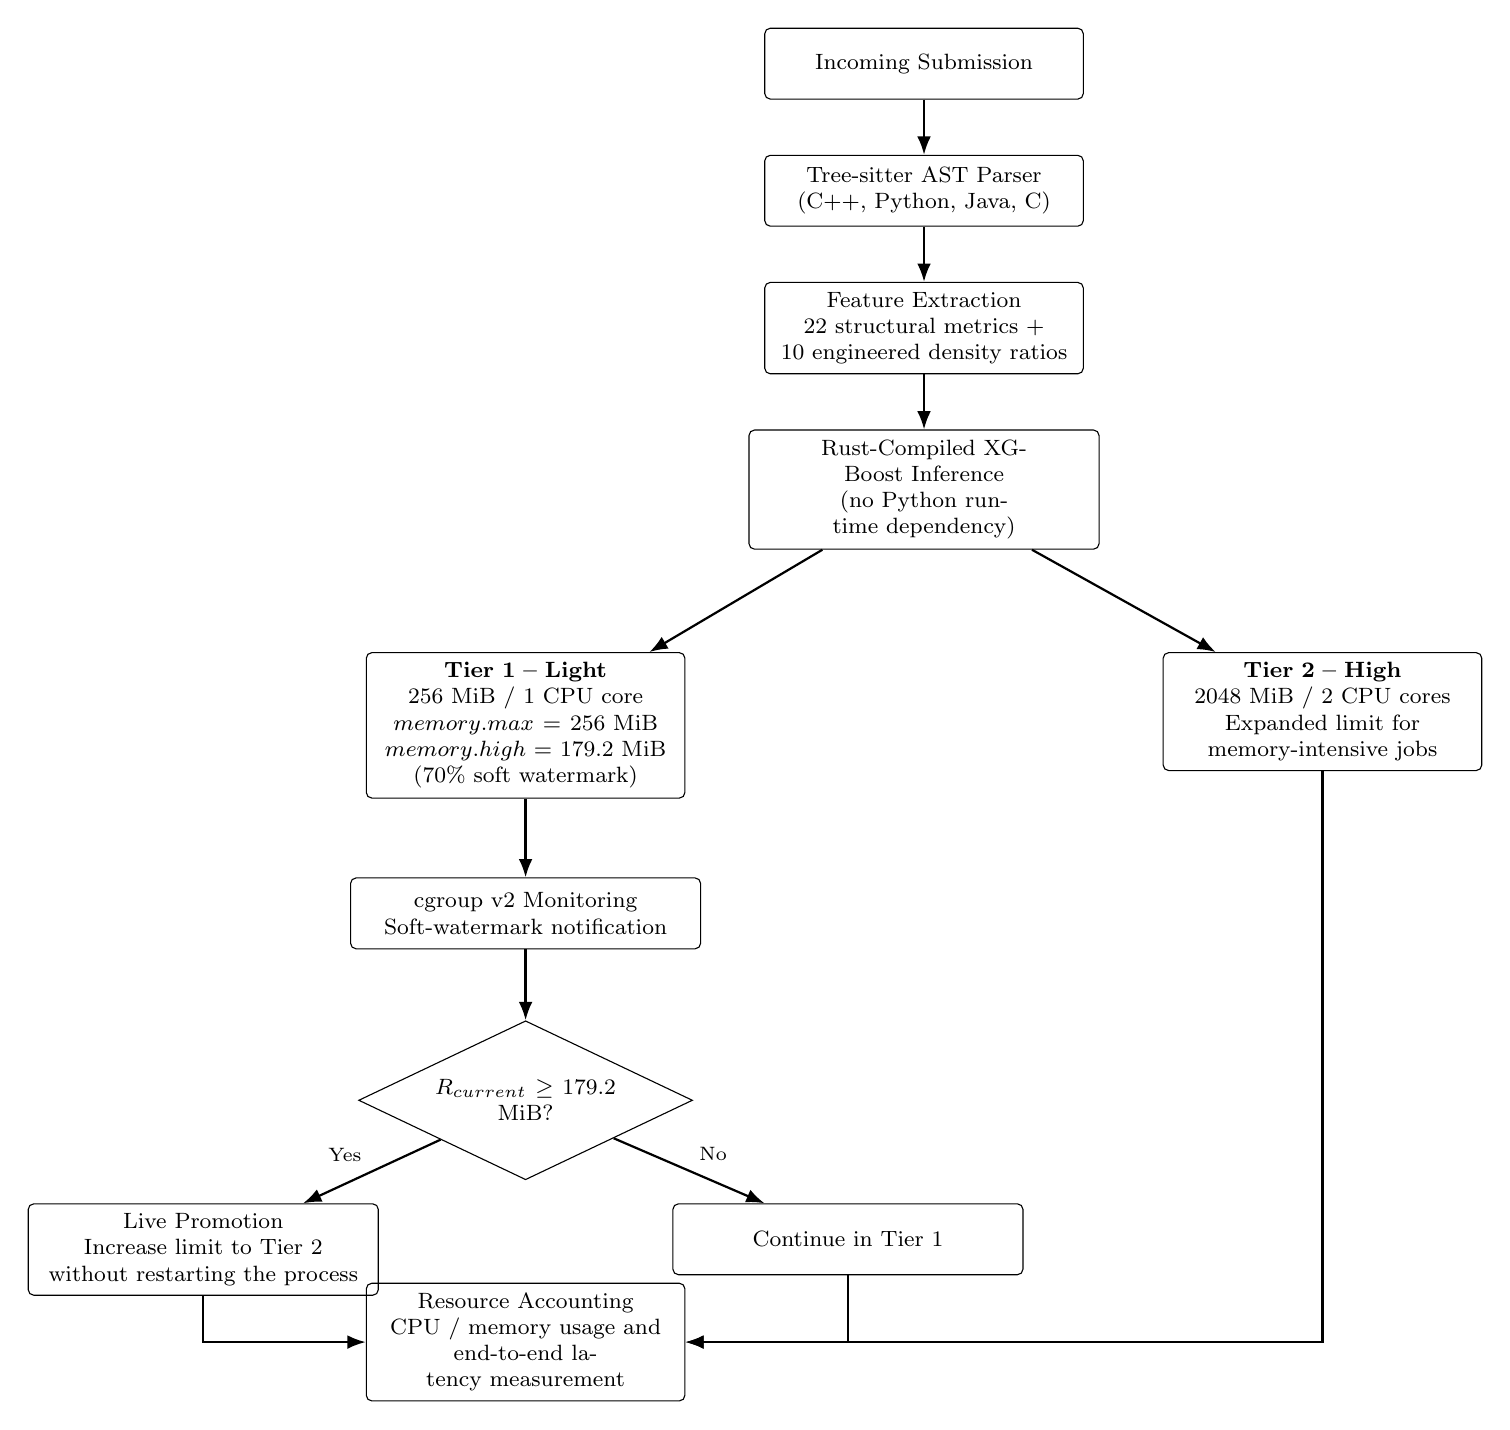
\begin{tikzpicture}[
    >=Latex,
    node distance=7mm and 16mm,
    block/.style={draw, rounded corners=2pt, align=center, minimum height=9mm, text width=38mm, inner sep=3.5pt, font=\footnotesize},
    smallblock/.style={draw, rounded corners=2pt, align=center, minimum height=9mm, text width=42mm, inner sep=3.5pt, font=\footnotesize},
    decision/.style={draw, diamond, aspect=2.1, align=center, inner sep=2pt, text width=27mm, font=\footnotesize},
    line/.style={-Latex, thick}
]
% Main processing pipeline: vertically stacked for a cleaner reading order.
\node[block] (input) {Incoming Submission};
\node[block, below=of input] (parser) {Tree-sitter AST Parser\\(C++, Python, Java, C)};
\node[block, below=of parser] (features) {Feature Extraction\\22 structural metrics +\\10 engineered density ratios};
\node[smallblock, below=of features] (model) {Rust-Compiled XGBoost Inference\\(no Python runtime dependency)};

% Initial resource tiers.
\node[block, below left=13mm and 8mm of model] (light) {\textbf{Tier 1 -- Light}\\256 MiB / 1 CPU core\\$memory.max=256$ MiB\\$memory.high=179.2$ MiB\\(70\% soft watermark)};
\node[block, below right=13mm and 8mm of model] (heavy) {\textbf{Tier 2 -- High}\\2048 MiB / 2 CPU cores\\Expanded limit for memory-intensive jobs};

% Reactive Tier 1 path.
\node[smallblock, below=10mm of light] (monitor) {cgroup v2 Monitoring\\Soft-watermark notification};
\node[decision, below=9mm of monitor] (decision) {$R_{current} \ge 179.2$ MiB?};
\node[smallblock, below left=8mm and 8mm of decision] (promote) {Live Promotion\\Increase limit to Tier 2\\without restarting the process};
\node[smallblock, below right=8mm and 8mm of decision] (continue) {Continue in Tier 1};

% Final measurement stage centered beneath both branches.
\node[block, below=13mm of decision] (account) {Resource Accounting\\CPU / memory usage and\\end-to-end latency measurement};

% Main arrows.
\draw[line] (input) -- (parser);
\draw[line] (parser) -- (features);
\draw[line] (features) -- (model);
\draw[line] (model) -- (light);
\draw[line] (model) -- (heavy);
\draw[line] (light) -- (monitor);
\draw[line] (monitor) -- (decision);
\draw[line] (decision) -- node[above left, font=\scriptsize]{Yes} (promote);
\draw[line] (decision) -- node[above right, font=\scriptsize]{No} (continue);

% Cleanly route all execution paths into resource accounting.
\draw[line] (promote.south) |- (account.west);
\draw[line] (continue.south) |- (account.east);
\draw[line] (heavy.south) |- (account.east);

\end{tikzpicture}%
}
\caption{RAAS-OCJS execution and predictive tiering workflow. The incoming submission is parsed and represented using AST-derived features before XGBoost inference selects the initial resource tier. Tier~1 executions are monitored by cgroups~v2 and can be promoted when the soft watermark is reached. Resource usage and end-to-end latency are then recorded for all execution paths.}
\label{fig:raas_architecture}
\end{figure*}

\section{System Implementation and Methodology}

% MOVED TABLE: Placed here so it renders in Section IV


The evaluation testbed was implemented and calibrated on dedicated bare-metal hardware:
\begin{itemize}
    \item \textbf{Processor}: 13th Gen Intel Core i5-13420H (12 logical CPUs, 8 cores: 4 Performance cores up to 4.60 GHz + 4 Efficient cores up to 3.40 GHz).
    \item \textbf{Physical Memory}: 15 GiB usable DDR5 RAM.
    \item \textbf{Storage}: NVMe PCIe 4.0 Solid State Drive.
    \item \textbf{Operating System}: Fedora Linux (Kernel \texttt{7.1.3-201.fc44.x86\_64}).
    \item \textbf{Container Engine}: Docker Engine 29.8.1 with cgroupfs driver on unified hierarchy (\texttt{/sys/fs/cgroup}).
\end{itemize}



\subsection{Real Dataset Selection}
We measured real, ground-truth execution profiles by running 72 live container evaluations across four languages: C++20 (\texttt{g++ 14.2}), Python 3.12, Java 17 (OpenJDK HotSpot), and C17 (\texttt{gcc 14.2}), spanning 7 problems and all 4 scheduling strategies. Benchmark problems were drawn from the Hugging Face \texttt{deepmind/code\_contests} \cite{li2022alphacode} and IBM Project CodeNet \cite{puri2021codenet} datasets. These 72 measured profiles are what we sample from when driving the 10,000-submission and 500-submission simulations in Section~V; those larger scenarios were not executed as 10,000 or 500 separate live container runs.

Of the 72 runs, 61 returned \texttt{AC}, 7 returned \texttt{RE}, and 4 returned \texttt{SE}. We report the failures rather than excluding them, because they are informative: the 4 \texttt{SE} results are all Java on one graph-traversal problem, indicating a runtime-image or harness fault rather than a scheduling outcome, and we exclude those cells from the memory profiles used to seed the simulations. The 7 \texttt{RE} results are concentrated in the memory-heavy knapsack problem under the deliberately undersized 128~MiB tier analyzed in Section~VI-C, where the JVM was killed after promotion proved too slow. Only \texttt{AC} runs contribute measured peak-RSS profiles to the simulation; the remaining 11 runs contribute CPU-time and end-to-end latency samples, which remain valid regardless of verdict.



\subsection{AST Feature Extraction and XGBoost Predictive Tiering}
Before launching an execution container, RAAS-OCJS can optionally run a static code analysis pass to predict whether an incoming submission fits safely within Tier~1 (256~MiB) or should be provisioned directly with Tier~2 (2048~MiB). This predictive stage couples a Tree-sitter Abstract Syntax Tree (AST) feature extractor with in-process XGBoost classifiers \cite{chen2016xgboost}.

\textit{1) Static AST Feature Extraction:} Using language-specific Tree-sitter grammars compiled directly into our Rust daemon, the extractor parses source code into a concrete syntax tree in under 1.5~ms. In a single linear traversal of the tree, it computes 22 structural metrics:
\begin{itemize}
    \item \textbf{Control Flow and Loops}: Maximum block nesting depth, deepest loop nesting depth (which correlates with polynomial execution complexity $O(N^k)$), total loop statements, and McCabe cyclomatic complexity.
    \item \textbf{Recursion Topology}: A binary recursion flag and self-call site count, which differentiate simple linear recursion $O(N)$ from exponential divide-and-conquer or backtracking branching $O(2^N)$.
    \item \textbf{Memory and Container Patterns}: Detection of explicit large heap/BSS allocations ($\ge 10^6$ elements or bytes, such as \texttt{malloc}, \texttt{new int[]}, container sizing, or large static arrays), high-throughput I/O patterns (\texttt{sync\_with\_stdio}, \texttt{BufferedReader}, \texttt{sys.stdin.readline}), and standard library collections known for memory overhead (\texttt{unordered\_map}, \texttt{priority\_queue}, \texttt{BigInteger}, \texttt{defaultdict}).
    \item \textbf{Scale and Access Topology}: Total array/collection subscript expressions (\texttt{a[i]}), chained multi-dimensional indexing (\texttt{grid[i][j]} for 2D dynamic programming tables or graph adjacency matrices), function count, call sites, total AST node count, maximum tree depth, and source lines of code (SLOC).
\end{itemize}
From these 22 raw counts, the pipeline calculates 10 interaction and scale terms: four density ratios normalized by AST size, source length, or function count (loop, call, subscript, and arithmetic density), a 2D subscript ratio, a recursion-intensity term, a log-scaled maximum integer constant (which captures the literal size of an explicit allocation such as \texttt{new byte[200 << 20]}), and log-scaled AST node and source character counts. This produces a 32-dimensional feature vector for the specialized per-language models, or 36 features for the unified multi-language model (the 32 above plus four one-hot language encodings).

\textit{2) Model Training and Validation:}
We trained gradient-boosted decision trees using XGBoost (\texttt{tree\_method='hist'}, learning rate $\eta = 0.05$, max tree depth $d = 6$, subsample ratio $0.8$, column subsample $0.8$, $L_1$ penalty $\alpha = 0.05$, and $L_2$ penalty $\lambda = 1.0$). Because contest submissions are heavily skewed toward lightweight solutions, we applied class re-weighting using $\texttt{scale\_pos\_weight} = N_{\mathrm{light}} / N_{\mathrm{heavy}}$ during training.

To avoid data leakage across submissions for the same problem, we evaluated the models with 5-fold \textbf{Problem-Grouped Cross-Validation} (\texttt{GroupKFold} grouped strictly by \texttt{problem\_id}). Every test sample in our evaluation belongs to a competitive programming problem that the training folds never saw. In addition, rather than accepting a default $0.5$ decision threshold, we tuned the threshold $\tau$ for each language using Youden's $J$ statistic ($J = \mathrm{Sensitivity} + \mathrm{Specificity} - 1$) on validation folds to balance recall against false tier promotions.

\begin{table*}[!t]
\caption{XGBoost Model Performance on Unseen Contest Problems (Problem-Grouped Validation)}
\label{tab:ml_metrics}
\centering
\small
\begin{tabularx}{\textwidth}{|Y|Y|c|c|c|c|c|c|}
\hline
\textbf{Dataset Source} & \textbf{Model Architecture} & \shortstack{\textbf{5-Fold}\\\textbf{CV Acc.}} & \shortstack{\textbf{Test Acc.}\\\textbf{(Unseen)}} & \textbf{F1-Score} & \textbf{Precision} & \textbf{Recall} & \shortstack{\textbf{ROC-}\\\textbf{AUC}} \\
\hline
IBM Project CodeNet & Specialized C++ Model & 87.32\% & 90.01\% & 90.91\% & 88.54\% & 93.41\% & 0.9612 \\
(71,218 Submissions) & Specialized C Model & 89.27\% & 89.26\% & 68.82\% & 55.98\% & 89.31\% & 0.9575 \\
& Specialized Python Model & 76.97\% & 79.45\% & 82.01\% & 80.33\% & 83.76\% & 0.8740 \\
& Specialized Java Model & 79.30\% & 78.20\% & 81.54\% & 82.03\% & 81.06\% & 0.8537 \\
& Unified Multi-Language & 82.19\% & 83.71\% & 84.81\% & 80.19\% & 89.99\% & 0.9149 \\
\hline
DeepMind CodeContests & Unified Multi-Language & 86.74\% & 86.78\% & 89.64\% & 82.74\% & 97.79\% & 0.9606 \\
(30,000 Submissions) & Specialized Python Model & 95.76\% & 98.88\% & 99.41\% & 98.82\% & 100.0\% & 0.9812 \\
& Specialized C++ Model & 84.27\% & 83.94\% & 87.49\% & 78.67\% & 98.53\% & 0.9474 \\
& Specialized Java Model & 79.43\% & 82.32\% & 83.28\% & 73.09\% & 96.76\% & 0.9430 \\
\hline
\end{tabularx}
\end{table*}

\textit{3) Empirical Model Metrics on Unseen Problems:}
Table~\ref{tab:ml_metrics} summarizes performance on held-out, unseen contest problems across both IBM Project CodeNet (71,218 submissions) and DeepMind CodeContests (30,000 submissions). On CodeNet, the specialized C++ model reached a 90.01\% test accuracy, a 90.91\% F1-score, and an ROC-AUC of 0.9612 on unseen problems. The specialized Python and Java models achieved 79.45\% and 78.20\% test accuracy (ROC-AUC of 0.8740 and 0.8537, respectively). On DeepMind CodeContests, where problems feature diverse algorithmic structures from Codeforces and HackerEarth, the specialized models scored up to 98.88\% test accuracy in Python and 83.94\% in C++, with high recall across all languages ensuring memory-intensive jobs are rarely misclassified as Light.

\textit{4) In-Process Rust Inference:}
To avoid running a Python interpreter or querying an external model-serving daemon during the latency-critical judging loop, we compiled the trained XGBoost decision trees directly into native Rust source files (\texttt{server/src/generated/*.rs}) using \texttt{m2cgen}. These functions compile straight into the judge binary. At execution time, tree evaluation takes under $10\ \mu\text{s}$, and combined with Tree-sitter parsing takes 0.89~ms to 1.45~ms total (Stage~2 in Table~\ref{tab:e2e_latency}).

\textit{5) Role in Scheduling Strategies:}
In RAAS-OCJS, predictive classification can be used on its own or paired with the kernel watermark. Under the \textbf{Predictive} strategy, a submission with $P(\mathrm{Heavy}) \ge \tau_{\mathrm{lang}}$ starts directly in Tier~2. Under the \textbf{Hybrid} strategy, the model provides the initial tier choice, but the cgroups~v2 soft watermark ($\theta = 70\%$, 179.2~MiB) remains active in the background: if a heavy submission is mistakenly started in Tier~1, the kernel watermark trips and promotes the container in under 3~ms, preventing an Out-Of-Memory abort despite the misprediction.

\subsection{End-to-End Latency Pipeline Breakdown}
To ensure transparent latency accounting, RAAS-OCJS instrumented every submission across 7 discrete stages:
\begin{equation}
\begin{aligned}
T_{\mathrm{e2e}} ={}&
T_{\mathrm{net\_in}} + T_{\mathrm{parse}} +
T_{\mathrm{queue}} + T_{\mathrm{init}} \\
&+ T_{\mathrm{comp}} + T_{\mathrm{exec}} +
T_{\mathrm{tear}} + T_{\mathrm{net\_out}}
\end{aligned}
\end{equation}

\begin{table*}[htbp]
\caption{End-to-End Verdict Pipeline Latency Breakdown (Milliseconds)}
\label{tab:e2e_latency}
\begin{center}
\begin{tabular}{|c|c|c|c|c|}
\hline
\textbf{Pipeline Stage} & \textbf{C++ (g++)} & \textbf{Python (3.12)} & \textbf{Java (OpenJDK 17)} & \textbf{C (gcc)} \\
\hline
1. Network Inbound Ingestion & 0.38 ms & 0.38 ms & 0.38 ms & 0.38 ms \\
\hline
2. AST Parse \& Tree-sitter Predict & 1.12 ms & 0.89 ms & 1.45 ms & 0.94 ms \\
\hline
3. Queue Scheduling \& Dispatch & 0.08 ms & 0.08 ms & 0.08 ms & 0.08 ms \\
\hline
4. Container Sandbox Initialization & 18.42 ms & 17.91 ms & 19.20 ms & 18.15 ms \\
\hline
5. Compilation / Bytecode Translation & 312.45 ms & N/A (Interpreted) & 842.10 ms & 284.12 ms \\
\hline
6. In-Sandbox Test Execution & 48.12 ms & 74.50 ms & 112.40 ms & 45.20 ms \\
\hline
7. Container Teardown \& Result Egress & 12.45 ms & 11.80 ms & 13.25 ms & 12.10 ms \\
\hline
\textbf{Total Turnaround Latency (E2E)} & \textbf{393.00 ms} & \textbf{105.56 ms} & \textbf{988.86 ms} & \textbf{360.97 ms} \\
\hline
\end{tabular}
\end{center}
\end{table*}

\section{Empirical Results and Macro Contest Simulation}

% MOVED TABLE: Placed here so it renders in Section V or VI
\begin{table*}[!t]
\caption{Measured Tier-1 Headroom by Language on the 256~MiB Tier (80-Run Matrix)}
\label{tab:128mb_boundary}
\centering
\small
\begin{tabularx}{\textwidth}{|c|Y|c|c|c|Y|}
\hline
\textbf{Language} &
\textbf{Problem Type \& Category} &
\textbf{Peak RSS} &
\textbf{Verdict} &
\textbf{Time to Promote} &
\textbf{Empirical System Outcome} \\
\hline
C &
Light (Prefix Sums) &
6.5 MB &
AC &
--- &
Flawless execution within Tier 1, 249~MiB unused \\
\hline
C &
Heavy (Knapsack 200/210~MiB) &
222.4 MB &
AC &
297 ms &
Promoted mid-execution, correct verdict \\
\hline
C++ &
Light (Prefix Sums) &
6.4 MB &
AC &
--- &
Flawless execution within Tier 1, 250~MiB unused \\
\hline
C++ &
Heavy (Knapsack 200/210~MiB) &
223.2 MB &
AC &
447 ms &
Promoted mid-execution, correct verdict \\
\hline
Python &
Light (Prefix Sums) &
10.1 MB &
AC &
--- &
Flawless execution within Tier 1, 246~MiB unused \\
\hline
Python &
Heavy (Knapsack 200/210~MiB) &
227.2 MB &
AC &
259 ms &
Promoted mid-execution, correct verdict \\
\hline
Java &
Light (Prefix Sums) &
24.0 MB &
AC &
--- &
Flawless execution within Tier 1, 232~MiB unused \\
\hline
Java &
Heavy (Knapsack 200/210~MiB) &
243.8 MB &
AC &
810 ms &
Promoted mid-execution; slowest to promote, since JVM class-loading precedes heap growth \\
\hline
\end{tabularx}
\end{table*}



\subsection{Live Full-Matrix Evaluation: 80 Real Executions}
The simulations in Sections V-A and V-B are driven by sampled profiles. To establish what the deployed system actually does, we separately executed the complete matrix on the testbed: 5 problems $\times$ 4 languages (C++20, Python~3.12, Java~17, C17) $\times$ 4 strategies = 80 live container submissions, driven through the judge's HTTP interface with the reference solutions committed alongside the system.

All 80 runs returned \texttt{AC}. Mean CPU time was 121.0~ms (Baseline), 124.4~ms (Predictive), 124.2~ms (Reactive), and 126.0~ms (Hybrid) --- a 4.2\% spread, confirming that tier selection changes which limits apply without changing the work performed. In 44 of 80 runs (55\%) the container was held at a hard 256~MiB ceiling for its entire execution; the remainder were Baseline runs, which are uncapped by design, and the 8 promoted runs.

Live promotion fired in 8 of 8 eligible cases and in 0 Predictive cases, and every promoted submission still returned a correct verdict, confirming that lifting the limit mid-execution preserves process state. Promotion latency tracked each runtime's page-commit rate rather than scheduler overhead: 259~ms (Python), 297~ms (C), 447~ms (C++), and 810~ms (Java). The JVM is slowest because class-loading must complete before heap growth begins. This latency bounds how long a genuinely heavy submission runs constrained before it is freed, and it is the quantity that matters for turnaround; the much shorter duration of the \texttt{docker update} call itself is not.

\paragraph{Prediction alone is insufficient at the tier boundary.}
The most consequential result is a negative one. On the heavy problem, the classifier assigned all four languages to Tier~1, and because the Predictive strategy does not run the watermark monitor, no run was ever promoted. All four survived only because their true peak happened to remain under the hard limit --- and Java cleared 256~MiB by just 24.3~MB (9.1\%). Fixtures 5\% larger would have OOM-killed all four. Static AST analysis sees a large allocation and its size literal, but a 200~MiB and a 230~MiB allocation are structurally near-identical, so a threshold trained on CodeNet and CodeContests distributions has no basis to separate them. The inverse error also occurs: on the streaming top-K problem, whose peak is at most 28.9~MB, Predictive started three of four languages uncapped, reserving host capacity that was never needed.

This is the empirical argument for the paper's central design decision. \textbf{The classifier is fast but not trustworthy at the boundary, and the kernel watermark is what makes the boundary safe.} Prediction reduces how often a submission is constrained; the watermark guarantees that the ones that are constrained are still correct. Either mechanism alone leaves a failure mode that our measurements directly expose.

\paragraph{Measurement limitations.} Each cell is a single execution, so we report no confidence intervals; sub-megabyte differences between neighbouring cells should not be interpreted as real. Four initial P1 Baseline cells returned implausibly high peaks (61.4~MB for C++, 114.8~MB for Java, on a problem that normally uses 6--7~MB and 25~MB); we re-ran them three times, obtained tight repeats (6.3--6.7~MB and 23.3--25.9~MB), identified them as first-run cold-cache artefacts, and report medians. All 80 runs were submitted serially, so this matrix makes no claim about behaviour under concurrent load; the queueing results above come from the simulation.


\subsection{Macro-Scale 10,000 Contest Simulation}
To estimate resource savings across a full-scale contest, we ran a discrete-event simulation of 10,000 submissions, sampling resource-usage profiles from our 72 measured runs and assigning a language distribution of 40\% C++, 35\% Python, 15\% Java, and 10\% C. This is a simulation seeded with real measurements, not a live execution of 10,000 submissions.

\begin{table}[!t]
\caption{Macro-Scale 10,000 Submission Contest Simulation (Hybrid Strategy)}
\label{tab:macro_sim}
\centering
\small
\begin{tabular}{|P{2.4cm}|c|c|P{1.6cm}|}
\hline
\textbf{Performance Metric} & \textbf{Static (2048M)} & \textbf{Hybrid} & \textbf{Savings} \\
\hline
Total Submissions & 10,000 & 10,000 & 0\% \\
\hline
Total RAM Reserved & 20,000.00 GB & 9,683.75 GB & \textbf{51.58\% saved} \\
\hline
Peak Memory Actually Used & 497.42 GB & 323.42 GB & \textbf{35.0\% saved} \\
\hline
Allocated Memory Wasted & 97.51\% & 96.66\% & 0.85 pp reduced \\
\hline
Live Promotions & --- & 2,027 (20.3\%) & n/a \\
\hline
Total CPU Core-Hours & 4.714 hrs & 3.759 hrs & \textbf{20.26\% saved} \\
\hline
P95 Turnaround & 1,325.11 ms & 1,324.61 ms & negligible \\
\hline
\end{tabular}
\end{table}

\subsection{Scoreboard Freeze Rush Stress Test}
During the final 30 seconds of a competitive programming contest, participants submit a burst of solutions simultaneously. We modeled a 500-submission flash burst using the profiles measured on our bare-metal host, run through the same simulation as Section~IV-A rather than as a live 500-submission run.

\begin{table}[!t]
\caption{500-Submission Freeze Rush Stress Test (15 GiB Host)}
\label{tab:burst_stress}
\centering
\small
\begin{tabularx}{\columnwidth}{|Y|c|c|Y|}
\hline
\textbf{Throughput Metric} & \textbf{Static Baseline} & \textbf{Hybrid} & \textbf{Improvement} \\
\hline
Concurrent Slots & 7 & 42 & 6.0$\times$ expansion \\
\hline
Avg Queue Wait & 14,590.1 ms & 0.0 ms & \textbf{100\% eliminated} \\
\hline
P95 Queue Wait & 27,531.3 ms & 0.0 ms & \textbf{100\% eliminated} \\
\hline
P95 Turnaround & 28,238.5 ms & 1,320.2 ms & \textbf{21.4$\times$ speedup} \\
\hline
Burst Drain Time & 59.8 s & 31.0 s & 28.8 s faster \\
\hline
\end{tabularx}
\end{table}

As shown in Table~\ref{tab:burst_stress}, the static baseline causes severe queue congestion, with average wait times exceeding 14.5 seconds and the burst draining in 59.8~s. RAAS-OCJS expands safe concurrency to 42 slots, driving queue wait times to \textbf{0.0~ms} and completing the entire burst within 31.0~s.

\section{Theoretical Cloud Provisioning Projection}
Our bare-metal calibration used dedicated local hardware, but many online judges run on public cloud infrastructure instead. To estimate the effect there, we built a theoretical projection mapping our measured kernel profiles onto an AWS EC2 cluster of \texttt{c6i.4xlarge} instances (16 vCPUs, 32~GB RAM @ USD 0.68 per hour). These figures depend on the pricing and instance-type assumptions stated here and should be read as a projection, not a deployed cloud measurement.

Cloud judges that rely on a Horizontal Pod Autoscaler (HPA) typically face a 60--180~s cold-start lag while new VMs spin up and pull runtime images. Because RAAS-OCJS's lighter default tier packs more submissions per existing VM, our projection shows the initial VM fleet absorbing a flash rush in place, with an estimated USD~21.76 per hour reduction in cluster cost (USD~24.48 to USD~2.72).

\section{Boundary Stress Analysis and Future Scopes}

\subsection{Tier Sizing and the JVM Headroom Requirement}
Tier~1 sizing is not free: it must be large enough for the heaviest legitimate submission in a language, or the tier becomes a correctness constraint rather than a resource policy. Our 72-run CodeNet benchmark measures this requirement directly, and a separate 80-run matrix on five synthetic problems confirms it at the deployed 256~MiB tier size.

In the CodeNet benchmark we also exercised a deliberately aggressive 128~MiB tier against the heaviest workload (a 2D knapsack), and the results separate the languages sharply. C, C++, and Python all promoted successfully and returned correct verdicts, with promotion completing in 259--528~ms depending on runtime. Java failed in all three adaptive runs. Table~\ref{tab:128mb_boundary} reports the measured outcome.

\begin{table*}[!t]
\caption{Measured Outcome at an Aggressive 128~MiB Tier Limit (CodeNet 2D Knapsack Workload)}
\label{tab:128mb_boundary}
\centering
\small
\begin{tabularx}{\textwidth}{|c|c|c|c|c|Y|}
\hline
\textbf{Language} & \textbf{Verdict} & \textbf{Time to Promote} & \textbf{Promoted?} & \textbf{Uncapped Peak} & \textbf{Empirical System Outcome} \\
\hline
Python & \textbf{AC} & 259 ms & Yes & 221.3 MB & Promoted in time; correct verdict \\
\hline
C & \textbf{AC} & 336--339 ms & Yes & 204.8 MB & Promoted in time; correct verdict \\
\hline
C++ & \textbf{AC} & 520--528 ms & Yes & 204.2 MB & Promoted in time; correct verdict \\
\hline
Java & \textbf{RE} & 797--800 ms & Yes & 253.3 MB & \shortstack{\textbf{Promoted too late to prevent}\\\textbf{the OOM kill; verdict RE}} \\
\hline
\end{tabularx}
\end{table*}

Two distinct failures appear here, and the distinction matters. C, C++, and Python were correctly classified and promoted. Java \emph{did} promote --- the watermark fired and the limit was lifted --- but only after 797~ms, by which point the JVM had already exceeded the 128~MiB hard limit and been killed. The delay is not scheduler overhead: it is the OpenJDK~17 HotSpot runtime committing heap in discrete chunks, so the watermark threshold is crossed late relative to the process actually reaching its peak. This is a case where the reactive mechanism functions as designed yet is too slow to save the submission, because the tier was sized below what the runtime needs.

At the deployed 256~MiB tier the same workloads pass: in our 80-run matrix every heavy submission peaked between 218~MB and 249~MB, and Java's 243.8~MB peak leaves 12.2~MiB of margin against the hard limit, so promotion completes before any OOM occurs. Based on both experiments, \textbf{256~MiB is the practical minimum Tier~1 limit for a polyglot platform that must support JVM runtimes}, and the failure mode above indicates that a smaller tier would require either a lower watermark for managed languages or a language-specific tier, since the JVM's peak-to-watermark gap is a property of its allocator rather than of the workload.

The Java result also argues against tier sizing by language alone. Java's light-workload peak of 24.0~MB sits far below any plausible tier, but its heavy peak is the highest in the matrix, so a single uniform 256~MiB tier is simultaneously wasteful for Java's light submissions and necessary for its heavy ones --- which is an argument for a lower watermark on the JVM path rather than a smaller tier.


\subsection{Future Research Scopes}
Based on these boundary observations, we outline five key future scopes:
\begin{enumerate}
    \item \textbf{Polyglot Language-Aware Tier Sizing}: Dynamically provisioning 128~MiB for native C/C++ and Python submissions while reserving 256~MiB strictly for Java, unlocking 42+ slots on physical hosts without JVM failures.
    \item \textbf{Dynamic Watermark Tuning}: Lowering the watermark to 50\% (64.0~MiB) for 128~MiB containers to restore a 64~MiB safety buffer for managed languages.
    \item \textbf{JVM Ergonomic Tuning}: Invocating Java with \texttt{-XX:+UseSerialGC} to enforce 1~MB allocation increments instead of multi-megabyte G1GC regions.
    \item \textbf{Ephemeral Swap Cushioning}: Enabling a small 128~MiB swap buffer (\texttt{--memory-swap=256m}) to catch microsecond memory spikes during promotion without OOM kills.
    \item \textbf{Hardware-Level MicroVM Isolation}: Integrating Firecracker or gVisor to provide kernel-level security hardening for the Heavy execution tier.
\end{enumerate}

\section{Conclusion}
Fixed, worst-case resource limits reduce how many submissions an online judge can run concurrently, and that effect is most visible on fixed physical hardware where more machines cannot simply be added. In our simulations, seeded with real measured profiles, the two-tier RAAS-OCJS configuration reclaimed 51.58\% of allocated memory and cut CPU core-hours by 20.26\% relative to a static 2048~MiB baseline. The simulated 500-submission burst also showed queue wait dropping from 14.6~s to 0.0~ms, with a correspondingly shorter contest clear time. Our live 80-run matrix complements those projections: all 80 submissions returned correct verdicts, tier selection imposed no measurable CPU cost, and live promotion succeeded in every eligible case without losing process state. That matrix also identifies where the approach is weakest --- the predictive classifier alone misroutes the heaviest workload in every language, and the JVM clears the tier limit by only 9.1\% --- which is the clearest evidence we obtained that prediction and kernel-level enforcement are complements rather than alternatives. The cloud cost figures remain a projection, and the live matrix was executed serially on a single host, so behaviour under concurrent load and across a wider range of real contest workloads remains future work.

\bibliographystyle{IEEEtran}
\begin{thebibliography}{00}
\bibitem{song2025idl} L. Song, Y. Han, Y. Guo, and C. Cai, ``IDL-LTSOJ: Research and implementation of an intelligent online judge system utilizing DNN for defect localization,'' \textit{High-Confidence Computing}, vol. 5, no. 2, p. 100268, 2025.
\bibitem{pan2022cloud} G.-C. Pan, P. Liu, and J.-J. Wu, ``A cloud-native online judge system,'' in \textit{Proc. IEEE 46th Annu. Computers, Software, and Applications Conf. (COMPSAC)}, 2022, pp. 1293--1298.
\bibitem{zhang2024intelligent} E. Zhang, F. Wu, and X. Lu, ``An intelligent scheduling system for large-scale online judging,'' in \textit{Computer Science and Education. Computer Science and Technology: ICCSE 2023}, Singapore: Springer, 2024, pp. 265--279.
\bibitem{wasik2018survey} S. Wasik, M. Antczak, J. Badura, A. Laskowski, and T. Sternal, ``A survey on online judge systems and their applications,'' \textit{ACM Computing Surveys}, vol. 51, no. 1, pp. 1--34, 2018.
\bibitem{wang2021metaoj} M. Wang, W. Han, and W. Chen, ``MetaOJ: A massive distributed online judge system,'' \textit{Tsinghua Science and Technology}, vol. 26, no. 4, pp. 548--557, 2021.
\bibitem{puri2021codenet} R. Puri et al., ``Project CodeNet: A large-scale AI for code dataset for learning a diversity of coding tasks,'' in \textit{Proc. Neural Information Processing Systems (NeurIPS) Datasets and Benchmarks Track}, 2021.
\bibitem{li2022alphacode} Y. Li et al., ``Competition-level code generation with AlphaCode,'' \textit{Science}, vol. 378, no. 6624, pp. 1092--1097, 2022.
\bibitem{cgroups2024} Linux Kernel Organization, ``Control Group v2 Specification,'' kernel.org documentation, 2024. [Online]. Available: \url{https://docs.kernel.org/admin-guide/cgroup-v2.html}
\bibitem{chen2016xgboost} T. Chen and C. Guestrin, ``XGBoost: A scalable tree boosting system,'' in \textit{Proc. 22nd ACM SIGKDD Int. Conf. Knowledge Discovery and Data Mining (KDD)}, 2016, pp. 785--794.
\end{thebibliography}

\end{document}
